\subsection{Протокол Эль-Гамаля}\index{протокол!Эль-Гамаля|(}
\selectlanguage{russian}

\begin{figure}
    \centering
    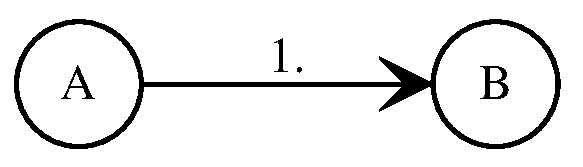
\includegraphics[width=0.5\textwidth]{pic/key_distribution-el-gamal}
    \caption{Взаимодействие участников в протоколе Эль-Гамаля\label{fig:key_distribution-el-gamal}}
\end{figure}

Протокол Эль-Гамаля (рис.~\ref{fig:key_distribution-el-gamal}, \cite{ElGamal:1984, ElGamal:1985}) за счёт предварительного распространения открытого ключа одной из сторон обеспечивает аутентификацию ключа для этой стороны. Можно гарантировать, что только владелец соответствующего закрытого ключа сможет вычислить сеансовый ключ. Однако подтверждение факта получение ключа (выполнение целей G1 и G8) не является частью протокола.

\begin{protocol}
    \item[(0)] Алиса и Боб выбирают общие параметры $p$ и $g$, где $p$ -- большое простое число, а $g$ -- примитивный элемент поля $\Z_p^*$.
    \item[{}] Боб создаёт пару из закрытого и открытого ключей $b$ и $K_B$:
        \[\begin{array}{l}
            b: 2 \leq b \leq p - 1, \\
            K_B = g^b \bmod p.
        \end{array}\]
    \item[{}] Открытый ключ $K_B$ находится в общем открытом доступе для всех сторон. Криптоаналитик не может подменить его -- подмена будет заметна.
    \item[(1)] Алиса выбирает секрет $x$ и вычисляет сеансовый ключ $K$
        \[ K = K_B^{x} = g^{bx} \bmod p. \]
        \[ Alice \to \left\{ g^x \bmod p \right\} \to Bob\]
    \item[(2)] Боб вычисляет сеансовый ключ
        \[ K = (g^x)^{b} = g^{bx} \bmod p. \]
\end{protocol}

Протокол не обеспечивает гарантию выбора нового сессионного ключа в каждом сеансе протокола (G10), а использование <<мастер>>-ключа $K_B$ для передачи сеансового ключа позволяет злоумышленнику вычислить все сессионные ключи из прошлых сеансов при компрометации закрытого ключа $b$ (цель G9).

\index{протокол!Эль-Гамаля|)}